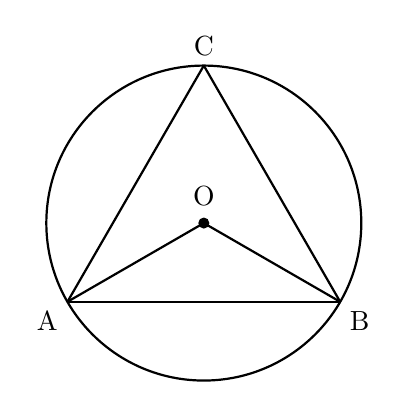
\begin{tikzpicture}[scale=1]

    % Define the radius of the circle
    \def\R{2}

    % Define the center of the circle O
    \coordinate (O) at (0,0);

    % Define points A, B, and C on the circle
    % C is placed at the top (90 degrees)
    % A and B are placed symmetrically at the bottom (210 and 330 degrees) to match the equilateral-like triangle in the image
    \coordinate (C) at (90:\R);
    \coordinate (A) at (210:\R);
    \coordinate (B) at (330:\R);

    % Draw the main circle
    \draw[thick] (O) circle (\R);

    % Draw the chords forming the inscribed triangle ABC
    \draw[thick] (A) -- (C);
    \draw[thick] (B) -- (C);
    \draw[thick] (A) -- (B);

    % Draw the segments connecting the center O to points A and B on the circle
    \draw[thick] (O) -- (A);
    \draw[thick] (O) -- (B);

    % Mark the center point O with a small filled dot
    \fill (O) circle (2pt);

    % Add the text labels for each point exactly as shown in the image
    \node[above] at (C) {C};
    \node[below left] at (A) {A};
    \node[below right] at (B) {B};
    \node[above] at (0, 0.1) {O};

\end{tikzpicture}